\Huge\textbf{Capitolo 9: \\Divisione cellulare}\\

\small
\section{Overview}
    Il ciclo cellulare è il processo per cui una cellula va incontro a una divisione tale per cui si ottengono in ultimo due cellule analoghe. Si divide in due fasi, l'interfase (I), e la mitosi (M). La fase I si divide in G0, G1, S e G2 (in G1, G2 e G3, G sta per \textit{gap}).\\
    Durante la fase S abbiamo la duplicazione del DNA e del centrosoma.\\
    Durante la fase M abbiamo l'effettiva separazione in due cellule figlie.\\
    Durante le fasi G1 e G2 abbiamo accrescimento del volume cellulare e dei suoi componenti. In G2 viene inoltre effettuata divisione mitocondriale.
    Divisione e duplicazione di organelli diversi da centrosoma e eventi diversi dalla duplicazione del materiale genetico sono meno critici per la cellula.
    
    \vspace{0.5cm}
    Il corpo umano è composto di circa $10^{14}$ cellule e ogni giorno se ne rigenerano circa $10^{12}$. Nel corso di una vita si assiste a circa $10^{16}$ divisioni cellulari. 
    Da questi numeri è facile intuire quanto questo processo debba essere controllato e preciso al fine di preservare la vita dell'organismo.\\
    Le componenti che determinano il corretto funzionamento del ciclo cellulare sono un \textit{clock} e un sistema di correzione degli errori (\textit{checkpoints}).
    
    \subsection{Divisione per cellule differenti}
        In tipologie di cellule differenti, velocità e caratteristiche del processo possono essere specifiche. In particolare:
        \begin{itemize}
            \item \textbf{divisione delle cellule embrionali in fasi precoci}:
                \begin{itemize}
                    \item sono divisioni che avvengono molto velocemente, da 30 a 60 minuti per divisione, questo perchè vengono saltate le fasi G1 e G2
                    \item non c'è accrescimento volumetrico delle cellule, sommando il volume occupato dalle figlie si ottiene lo stesso volume della cellula madre
                    \item non c'è controllo a livello di sintesi proteica, errori in questa fase causano la morte embrionale
                    \item il clock della situazione sono i processi di produzione, modificazione e degradazione delle proteine
                    \item non c'è trascrizione di mRNA
                \end{itemize}
            \item \textbf{somatiche}:
                \begin{itemize}
                    \item hanno un ciclo di circa 24 ore
                    \item questa duplicazione è sincronizzata all'accrescimento in volume
                    \item il controllo della produzione, modifica e degradazione delle proteine determina il clock biologico, assieme alla regolazione della trascrizione dell'mRNA.
                    \item è un processo molto controllato, la cellula può generare segnali per indicare il proprio suicidio
                \end{itemize}
            \item \textbf{embrione avanzato}:
                \begin{itemize}
                    \item le cellule interagiscono con l'ambiente
                    \item si differenziano in tessuti e organi diversi
                \end{itemize}
        \end{itemize}
        Le fasi G1 e G2 sono "accessorie": infatti nella fase embrionale precoce viene completamente saltata. G1 e G2 sono responsabili per l'accrescimento della cellula e per il "controllo qualità". \\
        Per controllo qualità si intendono degli eventi che avvengono per fare in modo che la duplicazione vada a buon fine, ovvero START, il controllo della duplicazione del DNA e l'allineamento dei cromosomi sulla piastra metafasica.
        \subsubsection{START}
            Uno dei controlli che viene effettuato dalla cellula a monte della sua divisione è controllare che siano disponibili una quantità sufficiente di sostanze nutritive. 
            Se questo controllo va a buon fine, allora si inizia la divisione senza più possibilità di tornare indietro (START è il punto di non ritorno). Nel caso le condizioni ambientali cambino dopo l'avvenuto START, la divisione avrà comunque luogo.
        \subsubsection{Controllo della replicazione del DNA}
            Il controllo dell'avvenuta e corretta replicazione del DNA viene effettuata durante la fase G2. Il processo richiede tempo in quando alcune regioni del DNA sono più difficilmente accessibili.
    
    \subsection{Definizioni e richiami}
        L'uomo possiede 23 coppie di cromosomi omologhi. \\
        Una cellula si dice aploide se ha una sola copia di ogni cromosoma, al contrario se ha due coppie di ogni cromosoma si dice diploide. \\
        Dopo la fase S, ogni cromosoma è composto da due cromatidi fratelli uniti a livello centromerico (esistono casi in cui sono uniti anche in altre zone).\\
        \begin{figure}[h]
            \centering
            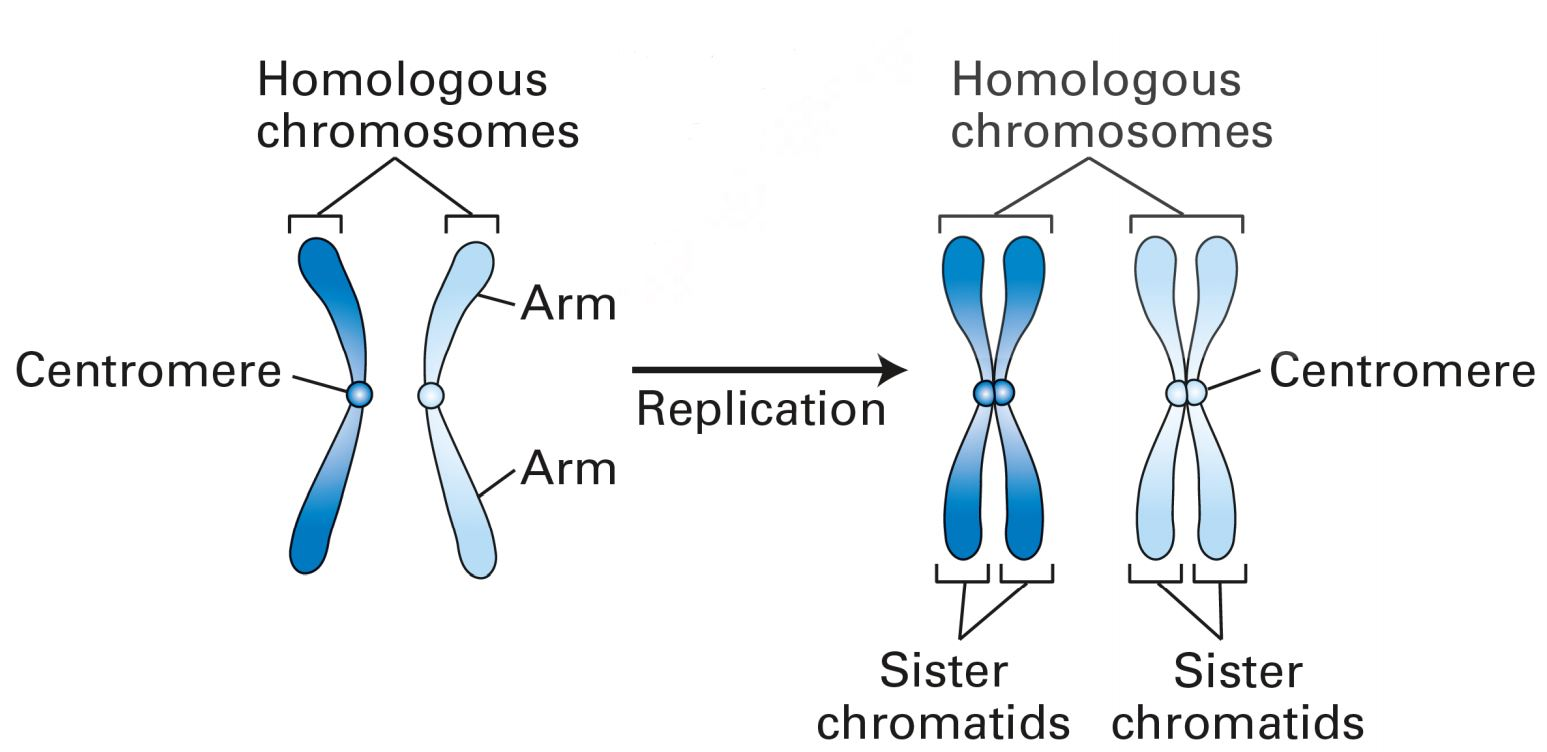
\includegraphics[width=0.5\textwidth]{images/cromosomiEcromatidi.JPG}
            \caption{\small Schema visuale della differenza tra cromosomi e cromatidi omologhi e fratelli}
            \label{fig:mesh1}
        \end{figure}
    
\section{Organismi modello e esperimenti}
    \subsection{SDS-PAGE}
        Per SDS-PAGE si intende un tecnica di elettroforesi di molecole associate a SDS, ovvero una molecola che conferisce carica negativa a quella di interesse.\\
        SDS sta per \textit{sodio dodecil solfato} ed è un detergente aggressivo che denatura le proteine e vi rimane associata, conferendo ad esse una netta carica negativa. Qualora uno stretch di AA sia più lungo saranno associate più SDS che conferiranno più carica.
        PAGE sta per \textit{poli acrilamide gel electrophoresis} ed è un gel composto da una miscela di acrilammide e biacrilammide che andranno a costituire una maglia di gel semi solido su cui le molecole target insieme a SDS potranno muoversi.
    
    \subsection{Esperimenti}
        \subsubsection{Hunt}
            Hunt conduce un esperimento utilizzando una sospensione di uova di riccio di mare, quindi cellule non attivamente ciclanti. 
            Induce la fecondazione delle uova simultaneamente introducendo gameti maschili con l'obiettivo di sincronizzare il ciclo cellulare tra le cellule uovo.\\
            Si introduce nella soluzione anche metionina marcata radioattivamente per poterla tracciare e rilevare.\\
            Hunt sottopose porzione dello stesso preparato a SDS-PAGE ogni 10 minuti con questo risultato:
            \begin{itemize}
                \item alcune proteine compaiono all'inizio del ciclo e continuano ad aumentare in quantità
                \item alcune proteine sembrano aumentare all'inizio del ciclo ma spariscono ritmicamente.
            \end{itemize}
            Perchè assumono questo comportamento ciclico, Hunt battezzò le seconde come \textit{cicline}. Hunt dedusse che le cicline controllassero in qualche modo la divisione cellulare. \\
            Ad oggi si sa che il clock che definisce il ciclo cellulare è composto da ciclina e CDK (ovvero chinasi ciclina dipendente). Il potere di questo complesso è quello di fosforilare proteine attivandole o inattivandole.
        
        \subsubsection{Kirschner}
            Kirschner condusse degli esperimenti utilizzando uova di anfibio perchè sono di grandi dimensioni (visibili anche ad occhio nudo) e vengono deposte in grandi quantità.\\
            Queste uova vengono trattate tramite un ormone che induce la meiosi (progesterone) e vengono quindi arrestate nel ciclo a valle, ovvero sono pronte al ciclo embrionale. \\
            Prelevando una quantità dal secondo preparato (trattato con progesterone) e inoculandola nel preparato iniziale, si nota che le cellule non trattate con ormoni cominciano anche esse a ciclare. \\
            Questo suggerisce l'esistenza di un fattore diffusibile che induce la divisione. \\
            Kirschner riesce inoltre ad isolare MPF, ovvero \textit{mitosis promoting factor} tramite tecniche di frazionamento del citoplasma.
        
        \subsubsection{Johnson e Rao}
            Questi due scienziati provarono a fondere una cellula in fase G1 con una in fase M. Il risultato fu che anche le cellule in G1 cominciano a compattare i loro cromosomi per prepararsi alla divisione. \\
            Questo esperimento conferma la presenza di MPF.
        
        \subsubsection{Hartwell}
            \textbf{Budding yeast}\\
                Budding yeas, ovvero \textit{Saccharomyces cerevisiae}, è un organismo eucariotico monocellulare utilizzato per molti esperimenti grazie al suo scarso costo, alla sua velocità di riproduzione e al peculiare fatto che consista di un ciclo aploide e uno diploide.\\
                La gemmazione è determinata da START, si possono dedurre le fasi cellulari dalla dimensione della gemma, la divisione finale non è equa in dimensioni (la cellula madre è più grande della figlia).\\
                
                
            Hartwell applicò una mutagenesi al lievito nella fase aploide. Tramite la tecnica del replica plate, riuscì a selezionare i mutanti temperatura sensibili. 
            Fece crescere questi mutanti prima a una temperatura permissiva e successivamente non permissiva.\\
            Riuscì in questo modo ad identificare CDC, perchè di fronte ad un arresto sincrono della divisione cellulare (\textit{cell division cycle}) e identificò anche geni e proteine che giocano ruoli importanti nel ciclo.\\
            Hartwell riuscì anche ad identificare i mutanti tramite la tecnica della complementazione. In particolare utilizzando delle librerie geniche, fu in grado di riconoscere CDC28 come mutante temperatura sensibile.\\
            Questa tecnica consiste nell'inserimento nel lievito di un plasmide con il gene di interesse e la successiva aggiunta del gene wt in oggetto.\\
            Nel momento in cui l'organismo viene traslato a una temperatura non permissiva solamente la coltura contenete CDC28 temperatura sensibile e CDC28 wt riesce a continuare il ciclo.\\
            In questo modo fu possibile isolare le sequenze wt di CDC28, che risulta essenzale per il passaggio dalla fase G1 alla fase S nel ciclo cellulare.
        
        \subsubsection{Nurse}
            \textbf{Schizosaccharomyces pombe}\\
                Schizosaccharomyces pombe è anche esso un lievito ma geneticamente molto distante da Saccharomyces cerevisiae preso in considerazione nell'esperimento precedente. 
                Questo lievito non effettua la duplicazione per gemmazione, ma dalla lunghezza della cellula si riesce comunque a dedurre in quale fase del ciclo cellulare si trova il lievito.\\
                
                
            Nurse condusse un esperimento usando il lievito Schizosaccharomyces pombe. In particolare rimpiazzò il gene CDC2 (analogo di CDC28 in Saccharomyces cerevisiae) con CDK1 (l'analogo per l'essere umano): il risultato fu che l'organismo preso in oggetto riesce comunque a effettuare la divisione cellulare sfruttando CDK1.
    
    \subsection{Proteine purificate}
        Esistono diversi metodi per ottenere delle proteine purificate, uno dei più utilizzati a livello laboratoriale consiste nel modificare una coltura batterica affinchè la produca selettivamente e ottenere eventualmente delle proteine ricombinanti.
        
        \subsubsection{Caratterizzazione}
        Per caratterizzazione della proteina isolata si intende \textit{in vitro kinase assey}.
        \begin{enumerate}
            \item introduzione di un accettore della fosforilazione, un substrato e CDC28
            \item introduzione ATP marcato con $P_{32}$ e protein chinasi
            \item con l'idrolisi di ATP, il gruppo fosfato marcato con $P_{32}$ viene trasferito sul substrato
            \item tramite SDS-PAGE e un autoradiogramma si può identificare la proteina radioattiva.
        \end{enumerate}
        Questo processo ha il fine di identificare e isolare la proteina.
        
        \subsubsection{Anticorpi specifici}
            In alternativa si possono produrre anticorpi specifici per una determinata proteina a partire da organismi complessi come i conigli. 
            Iniettando la proteina infatti l'organismo produce grandi quantità di anticorpi specifici che possono essere estratti e isolati.
            
        \subsubsection{Studio in modelli diversi}
            Avendo a disposizione l'anticorpo, si può sfruttare la reattività cross-specie per studiarlo indirettamente sull'uomo.
            \begin{enumerate}
                \item utilizzando cellule umane sincrone posso estrarre proteine in fasi differenti.
                \item con ogni estratto svolgo una SDS-PAGE. Si nota che alcune proteine sono sempre presenti, mentre alcune compaiono solamente dalla fase G2 in poi.
                \item con la tecnica del Western Blot (migrazione perpendicolare al gel di poliacrilammide per l'estrazione) si possono traferire le proteine su una membrana.
                \item utilizzando un anticorpo marcato precedentemente isolato per la proteina identifico in quale campione (quindi in quale fase) è presente la proteina target.
                \item tramite un immunoprecipitazione del complesso, utilizzando ATP radioattivo e facendo una SDS-PAGE posso individuare i complessi enzimaticamente attivi (utilizzo di ATP).
                \end{enumerate}
            Dalla prima fase di questo esperimento emerge che CDC28 (o CDC2 o CDK1) è sempre presente.\\
            Dalla seconda fase di questo esperimento (5.) emerge che CDC28 (o CDC2 o CDK1) sono enzimaticamente attive solo dalla fase G2 in poi. 
        
    \subsection{Esperimenti con ciclo cellulare}
        Con l'utilizzo di organismi modello e coltivazione di cellule umane tumorali (citiamo in particolare le cellule HeLa) è possibile studiare in specifico il ciclo cellulare.\\
        A livello morfologico, l'unica fase chiaramente identificabile è la fase M. Per questo motivo è necessario ricorrere ad altre tecniche per lo studio degli stadi.
            
        \subsubsection{Citometria di flusso}
            La \textit{citometria di flusso} (detta anche \textit{citofluorimetria} o \textit{FAX}) è un procedimento che a partire da una sospensione cellulare adeguatamente trattata riesce a differenziare le cellule in base alla fase mitotica in cui si trovano.\\
            Per fare questo la sospensione cellulare viene introdotta in un macchinario, il quale è in grado di isolare una cellula per ogni goccia. Queste vengono colpite da un raggio laser che induce fluorescenza.
            Un detector quantifica la fluorescenza.\\
            Utilizzando cellule di lievito e un fluoroforo per il DNA si evidenziano due picchi, uno un G1 e uno in G2: questo perchè le cellule in G1 (o in fasi precedenti, quindi una stessa quantità X di DNA) sono la maggioranza mentre il secondo picco corrisponde alla fase G2 in cui la quantità di DNA X raddoppia.
            Tra queste due misurazioni è visibile la fase S, intermedia, durante la quale il DNA si replica (quindi la quantità di fluorescenza è compresa tra X e 2X).
            \begin{figure}[h]
                \centering
                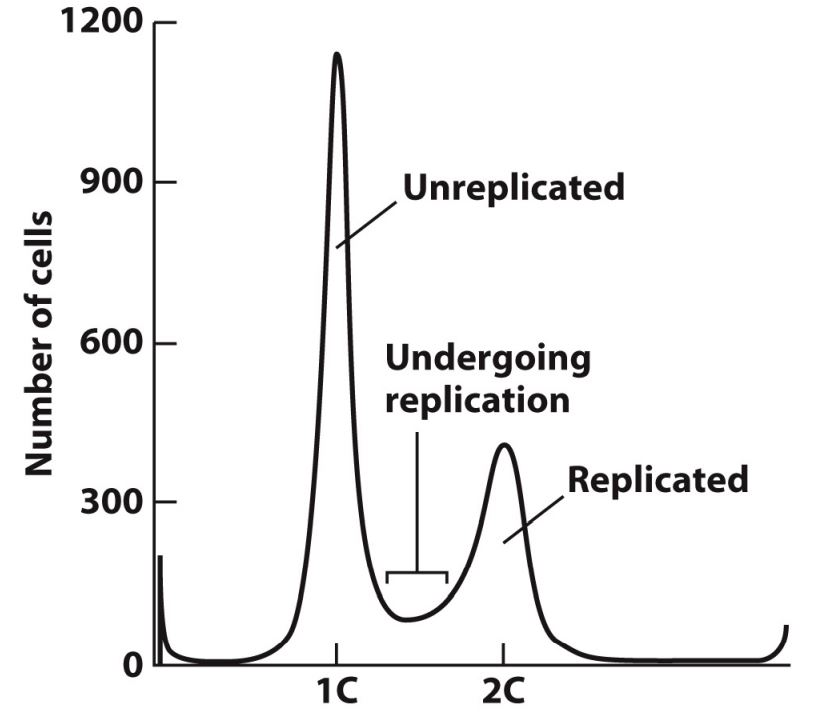
\includegraphics[width=0.5\textwidth]{images/citofluorimetria.JPG}
                \caption{\small Grafico di una citofluorimetria}
                \label{fig:mesh1}
            \end{figure}
            

\section{CDK e cilcine}
    \subsection{Struttura CDK}
        CDK consiste di un singolo peptide che presenta una struttura a tasca.  
        Presenta una porzione chiamata T-loop, un segmento proteico che contiene proteinchinasi: ha il ruolo di schermare l'ATP e la inattiva o attiva a seconda delle necessità.\\
        Il legame CDK e ciclina causa una riorganizzazione del T-loop che gli consente di fosforilare il substrato. per questo motivo CDK è \textit{ciclina dipendente}.
    
    \subsection{Funzioni, attivazione}
        CDK ha il compito di fosforilare proteine, in particolare gli AA target sono serina e treonina (anche la tirosina è spesso target di fosforilazioni ma CDK non se ne occupa). \\
        Esistono diversi complessi CDK-ciclina che sono attive in fasi diverse della divisione cellulare (quindi suddivisibili in G1-S, G2 e Mitosi).\\
        Le cicline vengono coinvolte in questo ordine: \textbf{D, E, A, B.}\\
        Se non interviene una ciclina, CDK non compie il suo dovere.
        
        \subsubsection{Cicline e CDK nell'uomo}
            Cicline (CIC) e CDK umane si associano secondo le seguenti coppie nel seguente ordine temporale. La stessa CIC si può associare a più CDK e allo stesso modo una CDK si può associare a più CIC.
            \begin{enumerate}
                \item CIC D + CDK 6 (per lo più durante fase G1)
                \item CIC D + CDK 4 (per lo più durante fase G1)
                \item CIC E + CDK 2 (G1, accompagna transizione in S)
                \item CIC A + CDK 2 (accompagna la fase S)
                \item CIC A + CDK 1 (comincia in G2, attività cresce sempre più fino alla fine di M)
                \item CIC B + CDK 1 (comincia in G2, attività cresce sempre più fino alla fine di M)
            \end{enumerate}
            Queste coppie non si limitano sempre a una sola fase del ciclo, ma possono "accompagnare" la transizione.
            
            \begin{figure}[h]
                \centering
                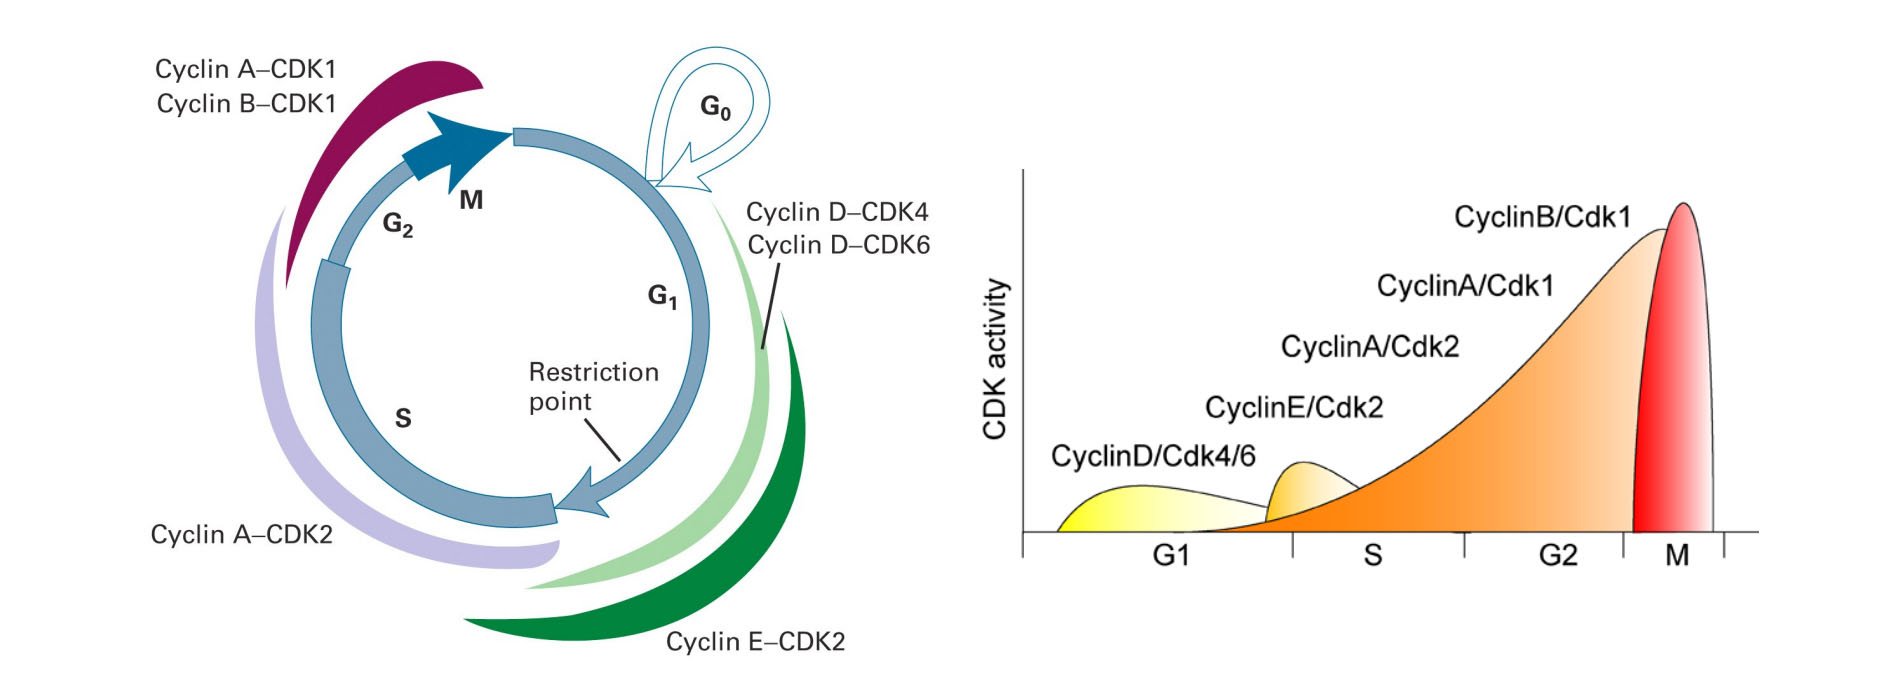
\includegraphics[width=1\textwidth]{images/CIC_e_CDK.JPG}
                \caption{\small A sinistra schema della presenza dell'attività CIC+CDK durante le fasi, a destra grafico della presenza dell'attività CIC+CDK}
                \label{fig:mesh1}
            \end{figure}
            
            La sommatoria delle attività CIC+CDK è un crescendo fino alla fine della mitosi stessa. Alcuni substrati possono essere fosforilati da qualunque CDK.\\
            Attraverso esperimenti su embrioni di topo, pare che CDK 1 sia sufficiente per svolgere l'intero ciclo cellulare e regolarne la divisione. Questo comporta comunque deficit e ritardi nello sviluppo ma suggerisce che l'unica CDK davvero fondamentale sia CDK 1.
            Si nota che è proprio la quantità di CDK che determina le fasi del ciclo cellulare. 
        
\section{Transizioni chiave}
        Le transizioni chiave nel ciclo cellualre sono le seguenti:
        \begin{enumerate}
            \item commitment alla divisione, ovvero START (restriction point)
            \item ingresso in M
            \item uscita da M
        \end{enumerate}
        
        \subsection{Punto di non ritorno}
            Start (per lievito) o Restriction point (per i mammiferi) rappresenta il punto di accesso al processo di divisione, dopo il quale non è possibile tornare indietro. Assume nomi diversi in organismi diversi.
            
            \subsubsection{Start}
                Il lievito decide o meno di entrare in divisione in base a \textit{ragioni metaboliche}. Vengono coinvolti SFB (fattore di trascrizione) normalmente inibito da Whi5. 
                \begin{enumerate}
                    \item Nel caso in cui i nutrienti per il metabolismo del lievito siano sufficienti, CDK viene attivata e Whi5 viene fosforilata e il fattore di trascrizione SFB diventa competente per produrre CDK.
                    \item La produzione di CIC 1 e 2 aumenta l'attività di CDK 
                \end{enumerate}
                \textbf{Il punto di non ritorno per questo sistema risiede nella fosforilazione del 50\% di Whi5.}
            
            \subsubsection{Restriction point}
                Allo stesso modo, esiste un fattore di trascrizione dei geni per le CIC, in questo caso chiamato E2F, inibito in condizioni normali da RB.
                \begin{enumerate}
                    \item In presenza di una concentrazione sufficiente di \textit{fattori di crescita}, CIC D e CDK 4 o 6 si attivano fosforilando RB.
                    \item Dissociandosi da RB, E2F permette la trascrizone di geni per la CIC E ed A. 
                    \item Le cicline appena prodotte si associano a CDK 2 e agiscono a loro volta fosforilando gli inibitori.
                \end{enumerate}
                \vspace{0.5cm}
                
            \begin{figure}[h]
                \centering
                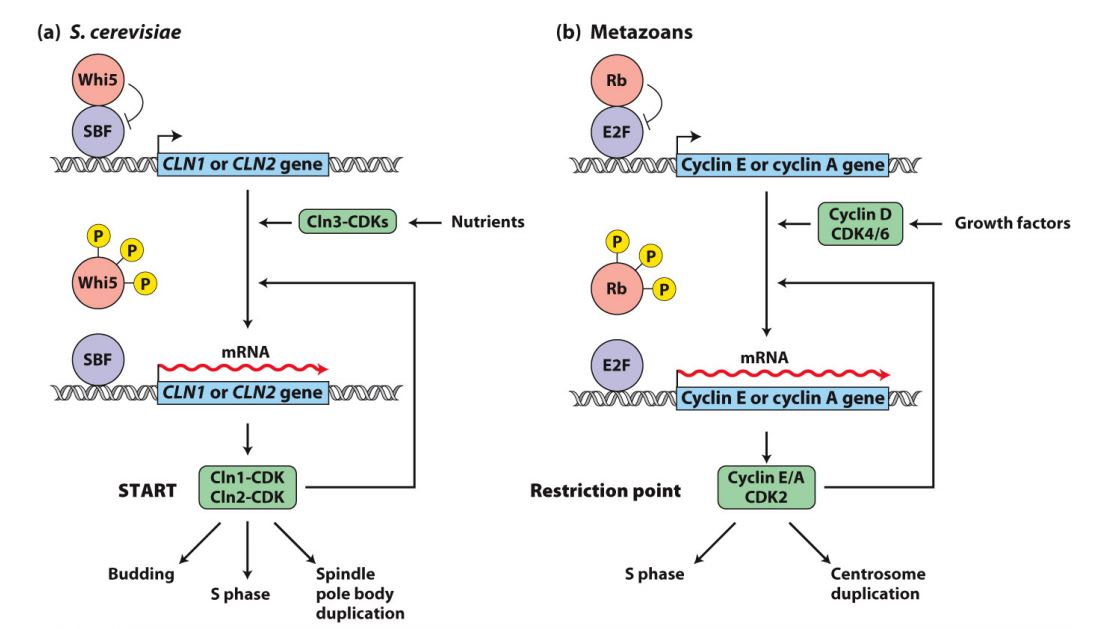
\includegraphics[width=1\textwidth]{images/start_e_restrictionPoint.JPG}
                \caption{\small A sinistra schema degli eventi si start nel lievito, a destra quelli in un mammifero}
                \label{fig:mesh1}
            \end{figure}
            
            Questi meccanismi fanno parte della categoria dei \textit{feedback positivi}, in quanto il prodotto agisce come agente attivante alla produzione di altro prodotto (si tratta quindi di un meccanismo di rinforzo).\\
            
            \textbf{CIC D}\\
                La CIC D in questo contesto è l'agente attivante per la fosforilazione di E2F.\\
            
            \textbf{E2F}\\
                E2F rappresenta una famiglia di fattori che attivano la trascrizione di CIC E ed A rimuovendo RB. Promuovono anche la sintesi di nucleotidi necessari alla duplicazione del DNA e attiva anche se stesso.\\
            
            \textbf{RB}\\
                Quando RB è fosforilato abbiamo il superamento del restricrion point. Contribuisce alla trascrizione di geni per le CIC o CDK1. Il passaggio del restriction point è legato all'attività di fosforilazione di CIC D e CDK 4-6.\\
                Mutazioni di RB possono causare una proliferazione incontrollata delle cellule, come succede nel retinoblastoma (RB). In altri casi ci possono essere degli oncogeni che veicolano segnali a CIC D + CDK 4-6 che fosforilano RB causando nuovamente una proliferazione incontrolalta.\\
                Le cellule HeLa non hanno RB.\\
            
            \textbf{Meccanismi di azione}\\
                Studi effettuati mediante IEF (iso elettro focalizzazione), hanno permesso di verificare in diversi stadi temporali il livello di fosforilazione di RB. In particolare è emerso che:
                \begin{itemize}
                    \item in cellule a cui non si forniscono fattori di crescita, tutta RB non è fosforilata (G0)
                    \item in cellule con bassi livelli di fattori di crescita, il 50\% di RB viene monofosforilata.
                    \item in cellule con alti livelli di fattori di crescita si avverte un salto improvviso della quantità di fosforilazioni. In particolare vengono effettuate 15 fosforilazioni (su serine o treonine) a partire da CIC E + CDK 2
                    \item Questa fosforilazione permane fino alla fine della fase M
                    \item Defosforilazione di RB e ripristino
                \end{itemize}
                
        \subsubsection{Fattori inibitori di CIC+CDK}
            La \textbf{CIC} è necessaria per l'attivazione delle chinasi CDK.\\
            La famiglia delle \textbf{INK4} (A, B, C, D) sono inibitori specifici del complesso CIC+CDK di fase G1 (citiamo p15, \textbf{p16}, p18, p19). \\
            Un altro gruppo di proteine ha attività inibitrici di CIC+CDK di cui fanno parte p21, \textbf{p27} e p57 che hanno azione su ogni CIC+CDK di ogni fase.\\
            
            \textbf{p16}\\
                p16 è un fattore che interviene in fasi precoci quindi risulta il più influente. In alcuni contesti, nell'organismo pluricellulare deve avvenire una differenziazione, la cellula non deve quindi proliferare.
                Per questo motivo viene espressa p16 la quale inattiva CIC D + CDK 4-6. \\
                La mutazione di p16 è generalmente legata all'insorgenza di tumori, poichè viene meno un meccanismo di contrasto all'iperproliferazione (ad esempio il melanoma multiplo).\\
                
            \textbf{SiC1}\\
                SiC1 è un fattore presente nel lievito che si lega alle CIC in fase S o precedenti. SiC1 \textit{non} fosforilata inibisce CIC+CDK di fase S ma non precedenti. \\
                SiC1 fosforilata (in sei siti differenti) da CIC+CDK (di fasi precedenti a S) causa la sua poliubiquinazione e la sua conseguente degradazione ad opera del proteasoma.\\
                Quindi a questo punto CDK di fase S sono libere di compiere la loro attività.\\
                
            \textbf{p27}\\
                p27 è un fattore che agisce su CIC D ed E. Il suo livello di attività (come in SiC1 per il lievito) è controllato dalla sua degradazione (poliUB e proteasoma). \\
                In particolare intervengono SCF complex (modula ubiquitin ligasi, \textit{Skip2 cullin F-box protein}, determina interazione con substrato), dei complessi generici che lavorano in funzione della fosforilazione. 
                Nel momento in cui p27 viene fosforilata, vengono legate le UB (il substrato più importante nel contesto umano) per la sua degradazione.
        
        \subsubsection{Regolazione della duplicazione}
            Per la regolazione della trascrizione de DNA, intervengono ORC (origin recognition complex), PRC (pre-replication complex) e MCM complex (minichromosome maintenance, un'elicasi che collabora in fase replicativa). Data una ORI, la replicazione comincia in base alla concentrazione delle CIC+CDK di fase S.
            \begin{enumerate}
                \item \textbf{G2, M}:\\
                in queste fasi ORC legano ORI sul DNA, non c'è interazione tra ORC e MCM complex poichè la fosforilazione di CDC 6 (o CTD 1) ne impedisce l'interazione. 
                Questa fosforilazione è operata dalle CIC+CDK di fase M.\\
                In queste fasi c'è un'\textbf{elevata} attività di CIC+CDK.
                \item \textbf{G1}:\\
                in questa fase avviene il caricamento del PRC sul DNA. Dopo il superamento del restriction point avvengono i seguenti eventi:
                \begin{enumerate}
                    \item CIC+CDK fosforilano un complesso facente parte di ORC e si apre una bolla replicativa
                    \item attivazione dell'elicasi
                    \item richiamo di altri fattori (come pCNA, ORCs ...)
                \end{enumerate}
                In questa fase l'attività CIC+CDK è \textbf{la più bassa possibile}.
                \item \textbf{S}:\\
                Replicazione. In questa fase l'attività di CIC+CDK è \textbf{alta}.
            \end{enumerate}
            La replicazione del DNA è quindi dettata dall'attività di CIC+CDK di fase S.\\
            Questa stessa sequenza di eventi è anche responsabile del fatto che ogni ORI venga replicata una e una sola volta in un ciclo.\\
            Durante la fase G1 sono già presenti gli anelli di coesina, alla fine della fase S questi stessi anelli intrappolano anche il filamento neosintetizzato.
            
            \begin{figure}[h]
                \centering
                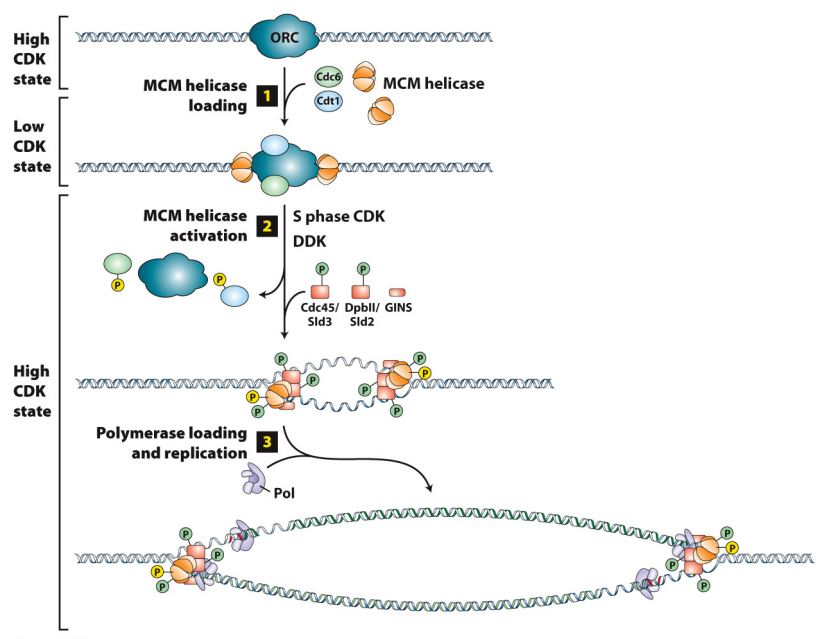
\includegraphics[width=0.8\textwidth]{images/regolazione_duplicazione.JPG}
                \caption{\small Schema della regolazione della duplicazione del DNA}
                \label{fig:mesh1}
            \end{figure}
        
    \subsection{Entrata in M}
        Profase, prometafase e metafase sono caratterizzate da un'\textbf{alta attività di CIC+CDK}.
        
        \subsubsection{Esperimento di Nurse}
            Paul Nurse, citato nei paragrafi precedenti, utilizzò S. pombe per i suoi studi. In particolare riuscì ad isolare dei mutanti temperatura sensibile del gene che codifica CDC2 (analogo di CDK1 nell'uomo).
            \begin{itemize}
                \item non mutanti: hanno una divisione normale
                \item mutanti di CDC2 recessivi : la cellula si allunga ma non si divide
                \item mutanti di CDC2 dominanti: la cellula entra in divisione precocemente.
            \end{itemize}
            Il gene CDC25 è presente anche in S.pombe e risulta estremamente conservato. Nurse osserva che:
            \begin{itemize}
                \item con un deficit di CDC25 ed eccesso di WHI1, la cellula si allunga e non si divide (analogo ai mutanti CDC2 recessivi)
                \item con un eccesso di CDC25 e un deficit di WHI1, la cellula di divide precocemente (analogo ai mutanti CDC2 dominanti)
            \end{itemize}
            Nurse ne dedusse che CDC25 funge da attivatore di CIC+CDC2 e WHI1 funge da inibitore dello stesso complesso (ricordo che S.pombe possiede un unica associazione CIC+CDC2). Questo funzionamento è conservato anche nei mammiferi.\\
            CDC25 è una fosfatasi mentre WHI1 una chinasi.
            
        \subsubsection{Sequenza eventi mitotici}
            \begin{enumerate}
                \item Wee1 fosforila la Tirosina15 di MPF inattivo (MPF = CIC+CDK). Wee1 è un inibitore.
                \item MPF inattivo viene fosforilato da CAK (cyclin activating kinase), in particolare viene fosforilata la treonina161 presente nel T-loop. Questa fosforilazione ha azione attivatoria.
                \item CDK raggiunge la sua piena attività con la fosforilazione della treonina161 e la presenza delle CIC
                \item CDC25 defosforila la tirosina15 di MPF (in particolare presente su CDK1). In questo modo il complesso MPF è effettivamente attivo.
            \end{enumerate}
            La defosforilazione operata da CDC25 è chiave per l'attivazione del complesso. La presenza di CDC25 è infatti pesantemente regolata per permettere l'attività corretta di MPF.
            
            \begin{figure}[h]
                \centering
                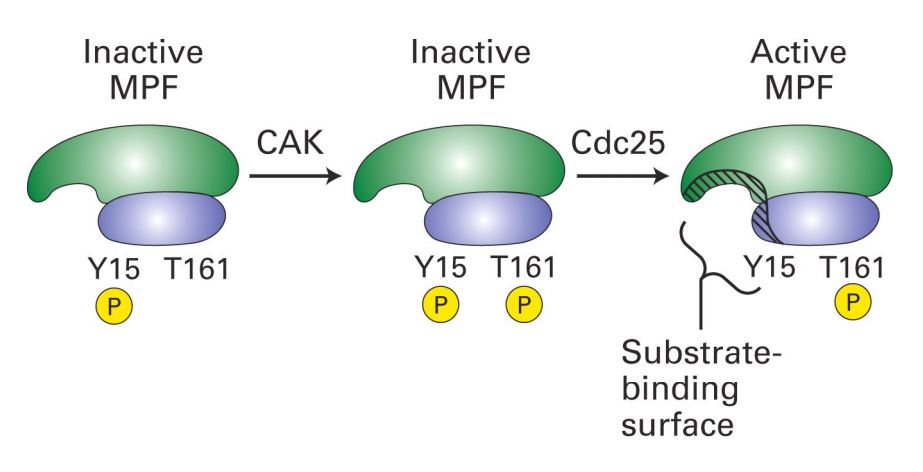
\includegraphics[width=0.5\textwidth]{images/MPF_activation.JPG}
                \caption{\small Schema dell'attivazione del complesso CIC+CDK tramite le fosforilazioni}
                \label{fig:mesh1}
            \end{figure}
            
        \subsubsection{Prime fasi della mitosi: Pro/Prometa/Metafase}
            La lamìna è un substrato per CDK1, quindi l'alto livello della sua attività contribuisce alla sua fosforilazione al 100\% e disassemblaggio. In questo modo abbiamo il dissolvimento della membrana nucleare. 
            Anche la condensazione dei cromosomi nella classica forma a X è dovuta all'alta attività di CIC+CDK.\\
            
            \textbf{Coesina e configurazioni}\\
                Gli anelli di coesina fino a questo punto erano presenti su tutta la lungehzza del cromosoma, ora duplicato. Con l'attivazione delle CIC+CDK di fase M abbiamo la fosforilazione degli anelli di coesina ad eccezione della zona centromerica.
                Questo è dovuto al fatto che in corrispondenza del centromero sono presenti delle proteine chiamate \textit{shugoshine} (dal giapponese "spirito guardiano"), che proteggono gli anelli di coesina dalla fosforilazione dando luogo alla caratteristica forma a X.\\
                I MT si associano al cinetocore con MAPS tramite una fosforilazione sempre ad opera di CIC+CDK di fase M.\\
                La configurazione finale che i cromosomi devono avere è detta \textit{anfitelica}, ovvero i MT associati al cinetocore sono in numero uguale su entrambi i cromatidi e sono provenienti da poli opposti della cellula. Altre configurazioni (merotelica, sintelica o monotelica) sono scorrette e causano un rallentamento della divisione. 
            
            \begin{figure}[h]
                \centering
                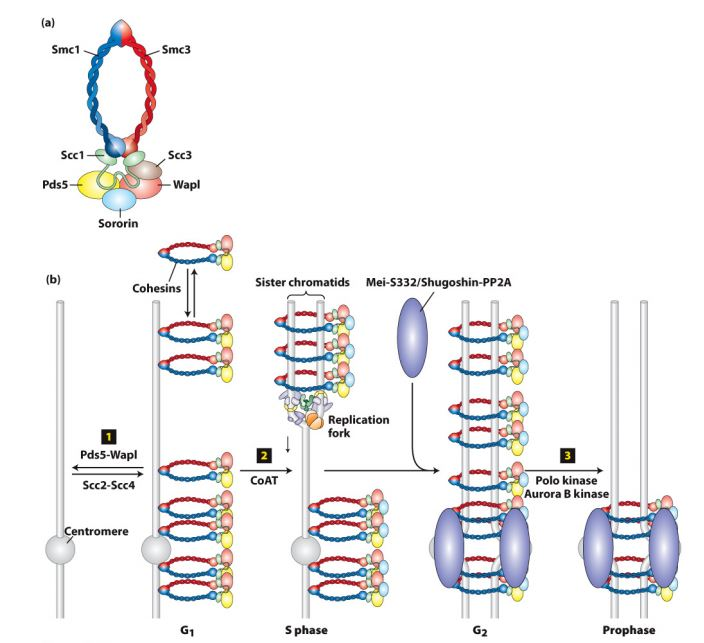
\includegraphics[width=0.8\textwidth]{images/shugoshina.JPG}
                \caption{\small Presenza della coesina in diversi momenti della divisione e azione della shugoshina}
                \label{fig:mesh1}
            \end{figure}
    
    \subsection{Uscita da M}
        Anafase e telofase sono caratterizzate da una \textbf{bassa attività CIC+CDK}. Il passaggio da metafase ad anafase è regolato dall'inibizione dell'attività CIC+CDK.\\
        L'anafase è indotta da un arresto improvviso dell'attività di CDK1 (da 100\% a 0\%).
        Il fattore responsabile per questo eventi è APC/C (anaphase promoting complex), il quale è responsabile della poliubiquitinazione di CIC B e della securina.\\
        \textbf{Gli attivatori di APC/C sono CDC20 e CDH1.}
        
        \subsubsection{CIC B}
            Target di APC/C è la CIC B, la quale viene poliUB e degradata dal proteasoma. Durante la transizione tra metafase e anafase, CDC20 determina l'interazione tra substrato e APC/C. 
            Eliminando CIC B, CDK non riesce più a svolgere la sua attività chinasica e vengono defosforilati i siti che precedentemente CDK1 aveva fosforilato per un "reset" dell'attività.\\
            CIC B viene poliUB tramite una D-BOX (dove D sta per destruction), ovvero una sequenza specifica per l'interazione CIC B e APC/C. In particolare è una sequenza di AA che permette il riconoscimento da parte di APC/C (R, x, x, L).\\
            Siccome la transizione tra metafase e anafase è dettata dalla degradazione della CIC B, si dice che questa transizione sia irreversibile. La degradazione della CIC B determina quindi il clock per la transizione di fase. 
        
        \subsubsection{Securina e separasi}
            Inizialmente la securina è associata alla separasi.
            APC/C ubiquitina la securina, la quale si distacca dalla separasi. La separasi singola è ora attiva e taglia determinate sequenze consenso di SCC1 (facenti parte della coesina). In questo modo i cromatidi fratelli sono liberi e la tensione ad essi associata li trascina verso poli opposti.
        
            \begin{figure}[h]
                \centering
                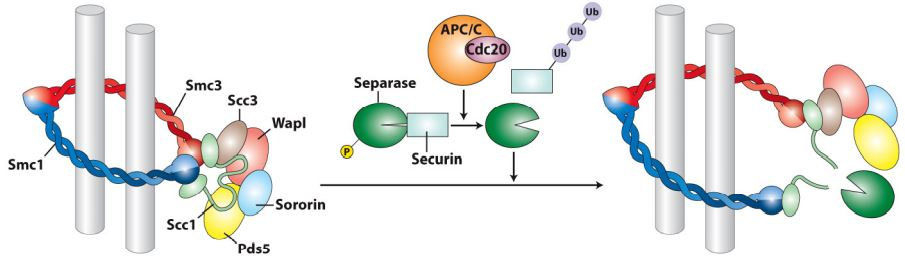
\includegraphics[width=0.6\textwidth]{images/securina_separasi.JPG}
                \caption{\small Azione della degradazione della securina}
                \label{fig:mesh1}
            \end{figure}
        
        \subsubsection{Ubiquitin-ligasi della mitosi}
            Le ubibuitin ligasi della mitosi sono regolate ed attivate attraverso fattori diversi. 
            Per esempio SCF fosforila il substrato il quale viene riconosciuto da F-BOX e successivamente poliUB, mentre ACP/C riconosce indipendentemente dalla fosforilazione la molecola a cui apporre UB ma esso stesso è regolato dalla fosforilazione.\\
            Quindi la stessa CDK1, l'oscillatore, promuove l'azione dei suoi inibitori.\\
            
            \textbf{ACP/C}\\
                APC/C è composto da 11 a 13 polipeptidi diversi e viene attivato tramite CDC20 oppure CDH1 (temporalmente in questo ordine).\\
                \begin{enumerate}
                    \item CDC20: è il fattore che inizia l'attivazione di APC/C ed è il più importante per l'attività regolatoria (in quanto comincia la degradazione della CIC B).
                    \item CDH1: è il fattore che interviene in un secondo momento e continua l'attività iniziata da CDC20, quindi mantiene basso il livello di CIC B durante le fasi finali di M e in G1. 
                \end{enumerate}
                ACP/C è controllato dalla fosforilazione. Per quanto riguarda la fosforilazione di CDH1: 
                \begin{itemize}
                    \item quando CDH1 si attiva, il livello di fosforilazione è basso
                    \item quando CDH1 si defosforila si associa a APC/C e continua l'azione di CDC20
                    \item quando CDH1 è altamente fosforilata determina l'inizio della mitosi con la sua dissociazione da APC/C. Si accumulano CIC di fase M e S. 
                    La fosforilazione di CDH1 è mantenuta tale dall'attività chinasica di CDK. 
                    Alla fine del processo viene ripristinata quindi defosforilata da una fosfatasi.
                \end{itemize}
                
                \begin{figure}[h]
                    \centering
                    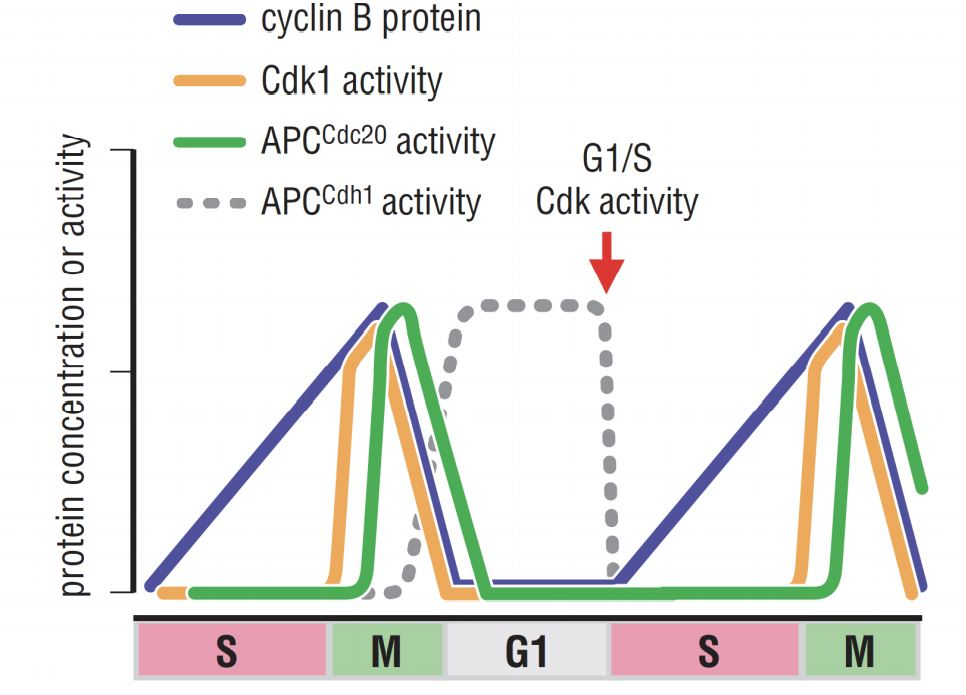
\includegraphics[width=0.6\textwidth]{images/attivita_APCC_CDC20_CDH1.JPG}
                    \caption{\small Grafico dell'attività di CIC+CDK in dipendenza dell'azione di APC/C con CDC20 e CDH1}
                    \label{fig:mesh1}
                \end{figure}
            
                Il picco di concentrazione di CIC B e di attività di CDK1 corrispondono (la presenza stessa di CIC B è necessaria per l'attività di CDK1). \\
                Quando inizia l'attività di APC/C dovuta a CDC20, sia l'attività di CDK1 che la presenza di CIC B diminuiscono drasticamente.\\
                Il delta temporale (*) tra il picco di attività di CDK1 e quello di APC/C con CDC20 è necessario alla mitosi, può aumentare nel caso in cui i cromosomi tardino ad allinearsi sulla piastra metafasica.\\
                L'attività di APC/C con CDH1 è presente in fase G1 per annullare l'attività di CIC B.
    
\section{Checkpoint}
    Il ciclo cellulare ha a disposizione una serie di meccanismi per il controllo del corretto funzionamento di varie fasi, in particolare si esprimono controllando l'oscillatore CIC+CDK. 
    Per la cellula è molto importante effettuare questi controlli perchè l'entrata scorretta in mitosi può portare ad eventi catastrofici. 
    
    \subsection{DNA damage response}
        La replicazione può essere soggetta a dei ritardi a causa di una rottura di un filamento, missmatch, impedimenti della forcella oppure danni ai nucleotidi.\\
        Per ritardare la divisione quindi intervengono dei fattori chiamati ATM e ART (uno dei due o in rapporto differente a seconda del danno) che sono due chinasi apicali per la risposta al danno al DNA.
        ATM e ATR fosforilano Chk1 e Chk2 (Chk sta per \textit{checkpoint}) che svolgono le seguenti azioni:
        \begin{enumerate}
            \item riparazione del DNA
            \item il segnale CDC25 viene fosforilato la quale azione ne causa la degradazione tramite il proteasoma
            \item attivazione di p21 (non si conosce il meccanismo) e fosforilazione di p53
        \end{enumerate}
        
        \subsubsection{p53}
            p53 è un fattore di trascrizione che, qualora sia fosforilato, determina la trascrizione di p21. p53 è un importante fattore per la soppressione dei tumori (circa il 50\% dei tumori presentano una mutazione di p53 e molti altri presentano degli impedimenti al suo corretto funzionamento).
            Per questo motivo p53 è detto guardiano del genoma. p53 è un effettore della DNA damage response essenziale, infatti controlla l'arresto del ciclo cellulare ed eventualmente l'apoptosi.\\
            
            \textbf{p53 nelle condizioni standard}\\
                Nelle condizioni normali, quindi senza stress, p53 ha basse concentrazioni perchè poliUB e degradata.\\
            
            \textbf{p53 nelle condizioni di stress}\\
                Nelle condizioni di stress, ovvero nel caso in cui avvengano danni al DNA quali una rottura di un filamento, missmatch, impedimenti della forcella oppure danni ai nucleotidi, attiva ATM e ATR, che a loro volta attiveranno Chk1 e Chk2.
                Questa cascata di attivazioni causa l'inibizione di MDM2 e la fosforilazione di p53. Quest'ultima inibisce l'associazione con MDM2. In complesso si previene la poliUB di p53.\\
                La presenza di p53 attiva determinate risposte, quali:
                \begin{itemize}
                    \item cambiamenti metabolici
                    \item sintesi di enzimi per il riparo del DNA
                    \item arresto in fase G1 o G2 (in base a quando avviene il danno) con attivazione di p21
                    \item senescenza con attivazione di p21
                    \item apoptosi
                    \item attivazione di MDM2 (questo per consentire la reversibilità del processo)
                \end{itemize}
                
                \begin{figure}[h]
                    \centering
                    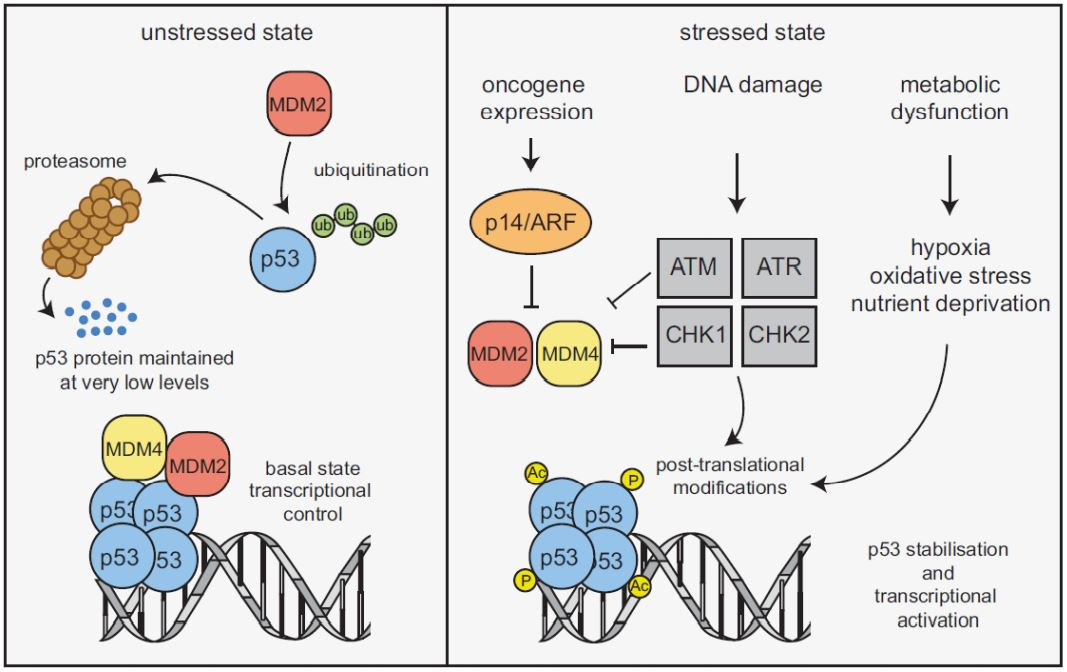
\includegraphics[width=0.8\textwidth]{images/p53.JPG}
                    \caption{\small p53 in condizioni normali e in condizioni di stress}
                    \label{fig:mesh1}
                \end{figure}    
        
    \subsection{Spindle assembly checkpoint}
        Lo spindle assembly checkpoint si occupa di controllare la corretta formazione della piastra mitotica, quindi il controllo della corretta bi-orientazione di tutti i cromosomi. \\
        Per dirsi bi-orientato, il cinetocore deve essere associato a MT provenienti da poli opposti in uguale numero, quindi la configurazione deve essere anfitelica. 
        Se così non fosse, le tensioni esercitate dai MT potrebbero non essere equilibrate e porterebbero i due cromatidi in posti diversi dalla piastra metafasica.
        Per questo motivo interviene \textit{Aurora B}, la quale chinasi fosforila porzioni del cinetocore provocando il distacco dei MT, quindi il reset del processo.\\
        Il delta temporale (*) varia proprio a seconda del tempo impiegato dai cromosomi a posizionarsi correttamente sulla piastra metafisica, includendo il tempo che potrebbe servire per correggere configurazioni erronee.
        In presenza di un solo cromosoma non correttamente bi-orientato si scatenano dei segnali che causano la posticipazione dell'anafase.\\
        
        SAC (spindle assembly checkpoint) controlla APC/C, nel caso ci siano cinetocori non correttamente associati ai MT, si genera un segnale in grado di posticipare l'inizio dell'anafase. Viene trascritto MAD2 (mitosis arrest defective) il quale è un inibitore alla transizione alla telofase.
        
        \subsubsection{MAD2}
            MAD2 ha la peculiarità di possedere due diverse conformazioni all'equilibrio, ovvero la conformazione open (MAD2-O) e la conformazione closed (MAD2-C). Nella conformazione MAD2-C è presente uno strech di AA che lega altre proteine. \\
            MAD2 contribuisce al signaling della scorretta associazione dei MT al cinetocore.
            \begin{enumerate}
                \item MAD2-C è legata a MAD1 (la quale possiede un recettore specifico sul cinetocore)
                \item MAD2 si associa a MAD1 nel momento in cui l'associazione MT-cinetocore non sia corretta (quindi diventa MAD2-C)
                \item MAD2-C causa la conversione del MAD2-O libero a MAD2-C associandolo a CDC20
            \end{enumerate}
            L'azione di MAD2 assomiglia a quella dei prioni, infatti una concentrazione di MAD2-C a contatto con MAD2-O causa un cambio di conformazione di quest'ultima a MAD2-C causando un feedback positivo.  \\
            Dal momento che MAD2-C lega CDC20, APC/C non viene attivato e non si entra in anafase.
        
            \begin{figure}[h]
                \centering
                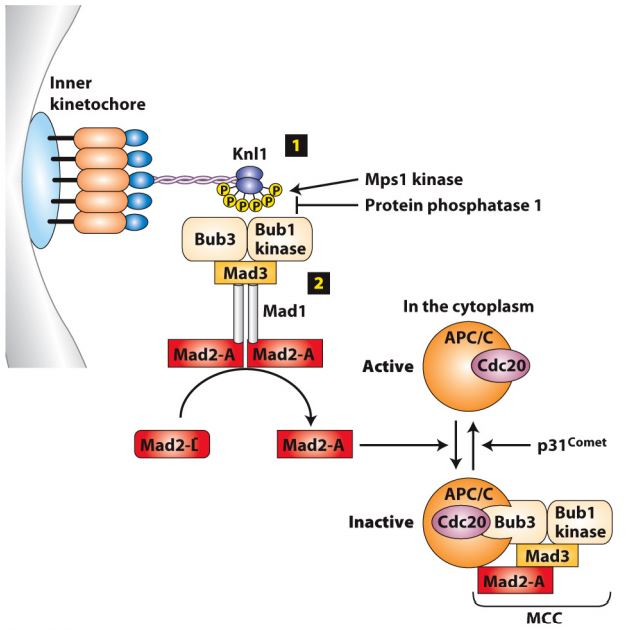
\includegraphics[width=0.6\textwidth]{images/MAD2.JPG}
                \caption{\small Azione di MAD2}            
                \label{fig:mesh1}
            \end{figure} 
    
\section{Morte cellulare}
    La morte cellulare può avvenire tramite percorsi differenti: apoptosi, necrosi, necroptosi.
    
    \subsection{Necrosi}
        La necrosi è il tipo di morte cellulare che ne determina il completo collasso. Avviene in risposta alla rottura della membrana e causa una fuoriuscita del suo materiale citosolico, può portare a infezioni. Corrisponde a un sabotaggio della cellula.
        
    \subsection{Necroptosi}
        La necroptosi è un comportamento caratterizzato da alcuni aspetti propri della necrosi e alcuni dell'apoptosi. 
    
    \subsection{Apoptosi intrinseca}
        L'apoptosi è la morte programmata di una cellula, è una caratteristica capacità della cellula, infatti è codificata da diversi geni. 
        Questo meccanismo è presente per favorire il ricambio cellulare, è importante per lo sviluppo embrionale (a livello embrionale le mani hanno un aspetto "palmato", successivamente le cellule che si che legano dita diverse si suicidano), è importante per il corretto sviluppo del sistema nervoso centrale (vengono prodotte cellule neuronali in eccesso e successivamente eliminate) e protegge dall'insorgenza dei tumori.
        
        \subsubsection{Aspetti caratteristici}
            \begin{enumerate}
                \item condensazione della cromatina
                \item contrazione del volume cellulare, arrotondamento e formazione di vescicole esterne dette corpi apoptotici
                \item distruzione del citoscheletro
                \item perdita dell'adesione ad altre cellule o ambiente extracellulare
                \item il contenuto citoplasmatico non fuoriesce e non causa infezioni
            \end{enumerate}
        
        \subsubsection{Fattori che inducono l'apoptosi}
            I fattori che fanno da star nel processo apoptotico sono le caspasi (CAS). Le caspasi sono una famiglia di proteasi che è caratterizzata da una cisteina nel proprio sito catalitico che riconosce un acido aspartico sempre presente al substrato.
            Non tutte le poteine della famiglia delle CAS sono deputate a questa funzione, ma alcune sono coinvolte nei processi infiammatori.\\
            Le CAS si divisono in caspasi esecutrici (CAS EXE) e caspasi iniziatrici (CAS INIT).\\
            \begin{figure}[h]
                \centering
                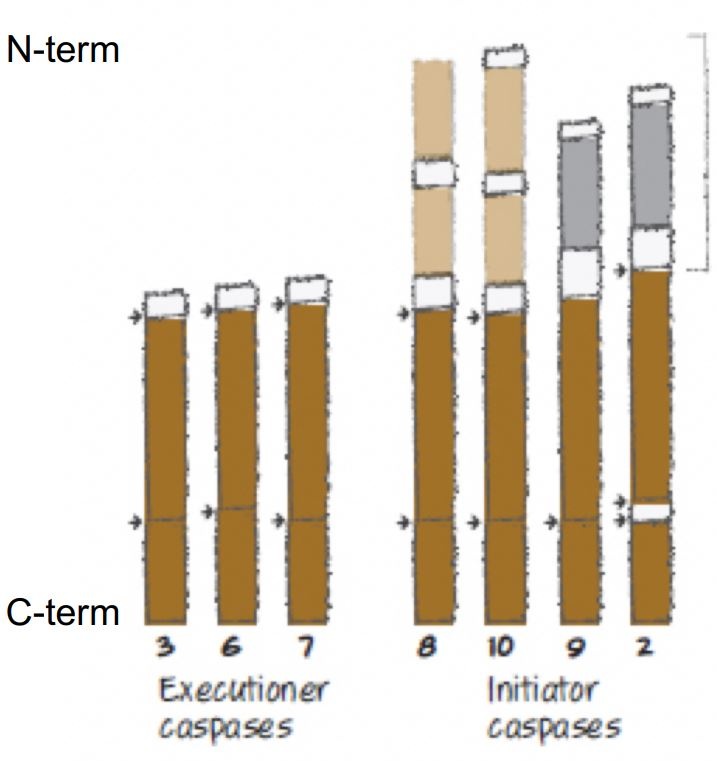
\includegraphics[width=0.4\textwidth]{images/caspasi.JPG}
                \caption{\small Divisione delle caspasi apoptotiche e confronto della relativa lunghezza}            
                \label{fig:mesh1}
            \end{figure} 
            
            \textbf{CAS iniziatrici}\\
                Le CAS INIT hanno una lunghezza in AA maggiore di quelle esecutrici. Presentano prodomini all'N-TERM. Ne fanno parte le \textbf{CAS 8, 9, 2.}\\
                Intervengono all'inizio del processo e determinano il punto di non ritorno per effettuare la procedura del suicidio.\\
            
            \textbf{CAS esecutrici}\\
                Le CAS EXE hanno una lunghezza inferiore e non presentano i predomini all'N-teminale. Sono processive e causano l'output proteolitico. Ne fanno parte le \textbf{CAS 3, 6, 7}.\\
                
            \textbf{CAS9}\\
                Le CAS9 svolgono la loro funzione grazie alla formazione di un complesso chiamato apoptosoma. Questo complesso è formato da tre peptidi differenti: CAS9, APAF1 e Citocromo C, ognuno presente in sette copie. La CAS9 diventa esecutiva nel momento in cui entra in contatto con altre CAS9. \\
                \begin{figure}[h]
                    \centering
                    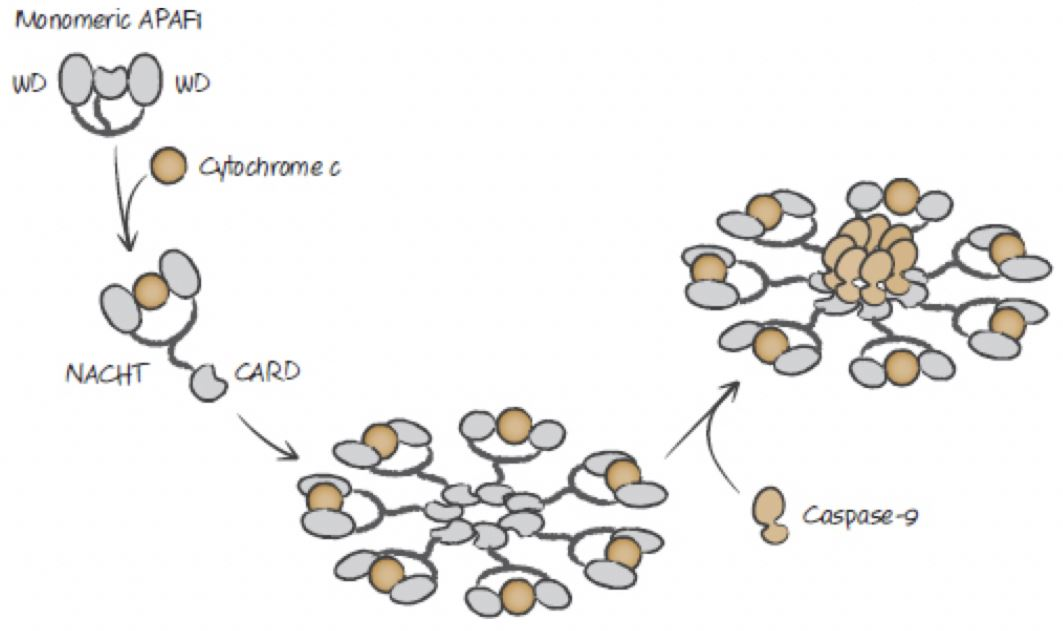
\includegraphics[width=0.5\textwidth]{images/apoptosoma.JPG}
                    \caption{\small Struttura e formazione dell'apoptosoma}            
                    \label{fig:mesh1}
                \end{figure} 
                L'elemento chiave per la formazione di questa struttura è il Citocromo C, che non è normalmente presente a livello citoplasmatico ma solamente nella porzione intermembrana dei mitocondri che solitamente collabora alla catena di trasporto degli elettroni. Il rilascio del Citocromo C nel citosol è necessario all'apoptosi.\\
                La conseguenza della formazione dell'apoptosoma è l'attivazione di CAS9 che esercita un'attività proteolitica nei confronti delle CAS EXE (3, 6, 7). Le CAS EXE possiedono una sequenza di AA riconosiuta da CAS9 che viene tagliata. In condizioni normali, le CAS EXE sono presenti a livello citoplasmatico ma si attviano solo qualora vengano proteolizzate.\\
                
            \textbf{Substrati di CAS EXE}\\
                Le CAS EXE agiscono su diversi substrati: 
                \begin{itemize}
                    \item iCAD: inibitore di CAD (caspase activated dnase), causandone l'attivazione, quindi il processo di segmentazione del DNA. 
                    \item flippasi e scramblasi: proteolizzano flippasi promuovendo l'equilibrio delle fosfatidilserine, mentre proteolizzando le scramblasi si attiva il flip-flop dei lipidi.\\
                    Perdendo l'asimmetria della concentrazione di fosfatidilserina, la cellula causa un signaling che viene intercettato dai globuli bianchi responsabili per la degradazione completa.
                \end{itemize}
                
        \subsubsection{Formazione apoptosoma}
            La formazione del complesso dell'apoptosoma è dovuto alla presenza delle BCL2 (B-cell lymphoma 2). Sono divise in tre gruppi: pro survival, pro apoptotiche BH3-only e pro apoptotiche con più domini BH.\\
            BH sono delle sequenze di AA specifiche, le BH3 sono comuni a tutte le BCL2.\\
            
            \textbf{BCL2 pro-apoptotiche: BAX e BAK}\\
                le BCL2 sono responsabili della formazione dei pori nella membrana del mitocondrio con la conseguente fuoriuscita di Citocromo C, necessario per la formazione dell'apoptosoma. BAX e BAK sono molto simili e hanno funzioni e meccanismi di attivazione analoghi.\\
                Normalmente BAX e BAK sono presenti a livello del citosol e rilocalizzano al mitocondrio nel caso sia necessario iniziare il processo apoptotico. In presenza di un segnale, BAX e BAK cambiano conformazione e oligomerizzano. 
                Oligomerizzando causano l'apertura di un foro nella membrana nucleare, la formazione di pori è chiamata MOMP (mitocondrial outer membrane permeabilization).\\
                Insieme alla fuoriuscita di Citocomo C, abbiamo la dispersione di Diablo e SMAC, altri componenti che inducono apoptosi.\\
                BAX e BAK sono solitamente inibite a livello citoplasmatico da altri elementi di BCL2 pro-survival (BCL2 stessa, BCL-XL, MCL1): sono gli stessi componenti famiglia delle BCL2 a inibire l'azione di altri componenti come BAX e BAK.\\
            
            \textbf{BH3 only}\\
                Le BCL2 BH3-only sono le proteine che rispondono effettivamente allo stimolo dello stress e possono agire tramite pathway di attivazioni diversi.\\ 
                In particolare possono attivare la cascata di sintesi di PUMA e NOXA, non normalmente presente ma prodotta grazie all'attivazione di p53. In concentrazione sufficiente di PUMA (o NOXA) si scatena l'apoptosi. \\
                Le BCL2 BH3-only possono attivare anche BAD la quale è regolata da una fosforilazione (se fosforilata è inattiva, altrimenti attiva), se attiva interferisce con l'azione delle BCM2 pro-survival.\\
                Bim è una proteina che è normalmente legata ai MT ma se quest'ultimo non risulta assemblato correttaemnte è disponibile a livello citoplasmatico e stimola le BCL2 HB3-only.
                \begin{figure}[h]
                    \centering 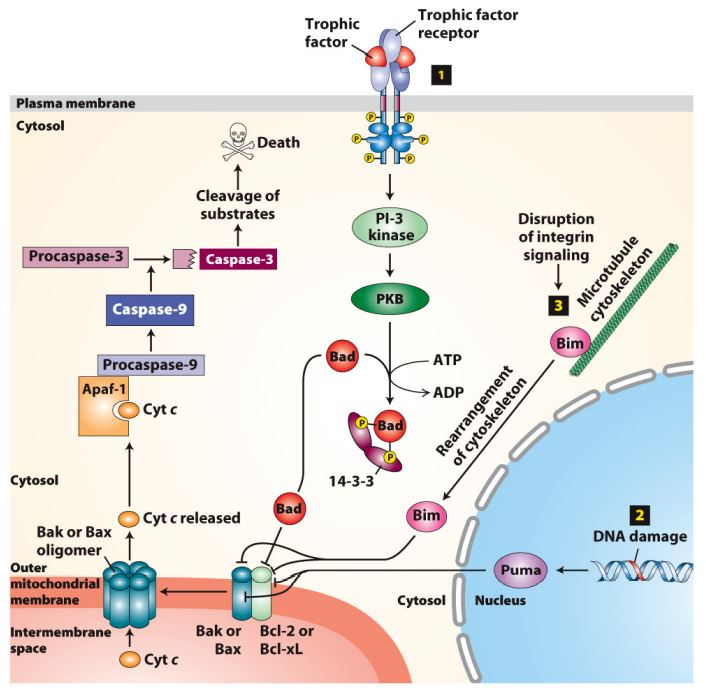
\includegraphics[width=0.8\textwidth]{images/pathway_BH3.JPG}
                    \caption{\small Pathway di stimolazione delle BCL2}            
                    \label{fig:mesh1}
                \end{figure} 
                
    \subsection{Apoptosi estrinseca}
        L'apoptosi estrinseca, a differenza della precedente, non decide autonomamente il suicidio ma questa azione è indotta da fattori esterni, per esempio cellule adiacenti o fattori estracellulari.\\
        L'esecuzione della procedura è analoga (si utilizzano sempre le CAS EXE) le quali però non vengono proteolizzate da CAS9, bensì da \textbf{CAS8}.\\
        
        \textbf{CAS 8}\\
            La CAS8 ha come substrati target le CAS EXE. L'attivazione di CAS8 è operata da DISC (death inducing signal complex), il quale determina l'assemblaggio di CAS8 e la sua dimerizzazione (con conseguente attivazione e proteolisi di CAS EXE). \\
            Tutto ciò è possibile attraverso un clustering dei recettori stimolati dal "ligando di morte". Il ligando di morte è rilasciato per esempio da linfociti.\\
            
        \textbf{BiD}\\
            BiD è una BCL2 BH3-only che può essere clivata da CAS8, aiuta l'apoptosi intrinseca. BiD è attivata in base a un azione proteolitica, con la perdita di uno stretch AA specifico viene attivata e si associa al mitocondrio.
            
        \begin{figure}[h]
           \centering 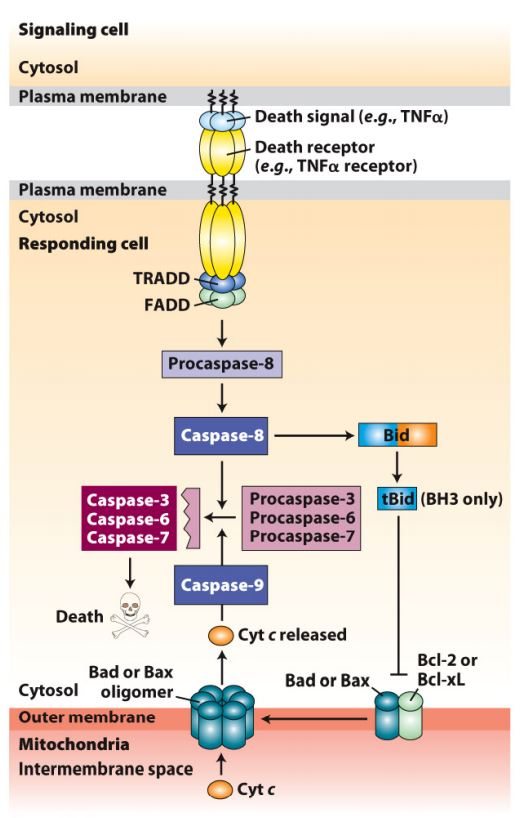
\includegraphics[width=0.5\textwidth]{images/CAS8.JPG}
           \caption{\small Pathway dell'attivazione di CAS8}            
            \label{fig:mesh1}
        \end{figure} 
        
    \subsection{CAS 2}
        La CAS 2 è una CAS INIT, la quale fino a poco tempo fa era poco compresa. Nel 2011 si è scoperto che il substrato target di CAS2 è MDM2: la separazione dei suoi due domini causa la dissociazione da p53 e impedisce la sua UB ligasi.\\
        Fisiologicamente, CAS2 è attivata dalla scorretta citochinesi la quale causa (tramite processi tuttora sconosciuti) la formazione del PiDDosoma e l'attivazione di p53. Pare che alla base della formazione del PiDDosoma ci sia la scorretta ripartizione dei centrosomi. 

\pagebreak